%%%%%%%%%%%%%%%%%%%%%%%%%%%%%%%%%%%%%%%%%
% Short Sectioned Assignment LaTeX Template Version 1.0 (5/5/12)
% This template has been downloaded from: http://www.LaTeXTemplates.com
% Original author:  Frits Wenneker (http://www.howtotex.com)
% License: CC BY-NC-SA 3.0 (http://creativecommons.org/licenses/by-nc-sa/3.0/)
%%%%%%%%%%%%%%%%%%%%%%%%%%%%%%%%%%%%%%%%%

%----------------------------------------------------------------------------------------
%	PACKAGES AND OTHER DOCUMENT CONFIGURATIONS
%----------------------------------------------------------------------------------------

\documentclass[paper=a4, fontsize=11pt]{scrartcl} % A4 paper and 11pt font size

% ---- Entrada y salida de texto -----

\usepackage[T1]{fontenc} % Use 8-bit encoding that has 256 glyphs
\usepackage[utf8]{inputenc}
%\usepackage{fourier} % Use the Adobe Utopia font for the document - comment this line to return to the LaTeX default

% ---- Idioma --------

\usepackage[spanish, es-tabla]{babel} % Selecciona el español para palabras introducidas automáticamente, p.ej. "septiembre" en la fecha y especifica que se use la palabra Tabla en vez de Cuadro

% ---- Otros paquetes ----

\usepackage{url} % ,href} %para incluir URLs e hipervínculos dentro del texto (aunque hay que instalar href)
\usepackage{amsmath,amsfonts,amsthm} % Math packages
%\usepackage{graphics,graphicx, floatrow} %para incluir imágenes y notas en las imágenes
\usepackage{graphics,graphicx, float} %para incluir imágenes y colocarlas

% Para hacer tablas comlejas
%\usepackage{multirow}
%\usepackage{threeparttable}

%\usepackage{sectsty} % Allows customizing section commands
%\allsectionsfont{\centering \normalfont\scshape} % Make all sections centered, the default font and small caps

\usepackage{fancyhdr} % Custom headers and footers
\pagestyle{fancyplain} % Makes all pages in the document conform to the custom headers and footers
\fancyhead{} % No page header - if you want one, create it in the same way as the footers below
\fancyfoot[L]{} % Empty left footer
\fancyfoot[C]{} % Empty center footer
\fancyfoot[R]{\thepage} % Page numbering for right footer
\renewcommand{\headrulewidth}{0pt} % Remove header underlines
\renewcommand{\footrulewidth}{0pt} % Remove footer underlines
\setlength{\headheight}{13.6pt} % Customize the height of the header

\numberwithin{equation}{section} % Number equations within sections (i.e. 1.1, 1.2, 2.1, 2.2 instead of 1, 2, 3, 4)
\numberwithin{figure}{section} % Number figures within sections (i.e. 1.1, 1.2, 2.1, 2.2 instead of 1, 2, 3, 4)
\numberwithin{table}{section} % Number tables within sections (i.e. 1.1, 1.2, 2.1, 2.2 instead of 1, 2, 3, 4)

\setlength\parindent{0pt} % Removes all indentation from paragraphs - comment this line for an assignment with lots of text

\newcommand{\horrule}[1]{\rule{\linewidth}{#1}} % Create horizontal rule command with 1 argument of height

\graphicspath{ {./images/} }
\usepackage{subcaption}
\usepackage{hyperref}
\usepackage{soul}

%----------------------------------------------------------------------------------------
%	TÍTULO Y DATOS DEL ALUMNO
%----------------------------------------------------------------------------------------

\title{	
\normalfont \normalsize 
\textsc{\textbf{Inteligencia de Negocio (2018-2019)} \\ Doble Grado en Ingeniería Informática y Matemáticas \\ Universidad de Granada} \\ [25pt] % Your university, school and/or department name(s)
\horrule{0.5pt} \\[0.4cm] % Thin top horizontal rule
\huge Memoria Práctica 1: \\Análisis Predictivo Empresarial Mediante Clasificación. Grupo de Prácticas 1 \\ % The assignment title
\horrule{2pt} \\[0.5cm] % Thick bottom horizontal rule
}

\author{Luis Balderas Ruiz \\ \texttt{luisbalderas@correo.ugr.es}} 
 % Nombre y apellidos 


\date{\normalsize\today} % Incluye la fecha actual

%----------------------------------------------------------------------------------------
% DOCUMENTO
%----------------------------------------------------------------------------------------

\begin{document}

\maketitle % Muestra el Título

\newpage %inserta un salto de página

\tableofcontents % para generar el índice de contenidos

\listoffigures

\listoftables

\newpage


%----------------------------------------------------------------------------------------
%	Introducción
%----------------------------------------------------------------------------------------

\section{Enlace al proyecto e Introducción}

\href{https://consigna.ugr.es/f/tsFMHLeXJihLASdx/P1-Balderas-Ruiz-Luis.zip}{Aquí puedes encontrar el proyecto KNIME} \\


En esta práctica tratamos de resolver un problema de clasificación, basado en \cite{main-article}, donde se presenta un sistema de apoyo a la decisión dedicado a predecir la popularidad de noticias en la red. Para ello, se examinan una gran cantidad de características (keywords, número de tokens, día de publicación...) a través de un IDSS (Intelligent Decision Support System) específico, un ABI (Adaptitve Business Intelligence), donde se combina predicción y optimización, de forma que, utilizando modelos que predigan con una cierta probabilidad qué noticias serán populares antes de que se publiquen y poder tomar decisiones óptimas en función de ese conocimiento extraído. Sin embargo, nuestro experimento, llevado a cabo sobre un dataset de 39000 noticias, consistirá en utilizar distintos clasificadores sobre el conjunto de datos etiquetado y compararlos. Más tarde, se tratará de mejorar los resultados mediante técnicas de preprocesamiento o ajuste de parámetros. En dicho preprocesamiento será necesaria la utilización de técnicas de visualización. \\

Entre los clasificadores disponibles, utilizo Random Forest (RF), Gradient Boosted, SVM, KNN, Naïve-Bayes, C4.5 de KNIME y Red Neuronal. Los he elegido por su distinta variedad así como por las recomendaciones dadas en \cite{choosing1} y \cite{choosing2}. Utilizo \cite{data_mining_book} como libro de referencia y la documentación de la asignatura aportada en clase de teoría. Por último, quiero señalar que algunos de esos algoritmos necesitan normalización, eliminar variables categóricas o algún tratamiento de \textit{missing values}. En esos casos, para la primera ejecución, se hará el mínimo tratamiento posible de los datos, pudiéndo enriquecerse y extenderlo en las siguientes etapas del estudio.



%----------------------------------------------------------------------------------------
%	Resultados obtenidos
%----------------------------------------------------------------------------------------

\section{Resultados obtenidos}

\subsection{C4.5 KNIME}

\begin{figure}[H] %con el [H] le obligamos a situar aquí la figura
	\centering
	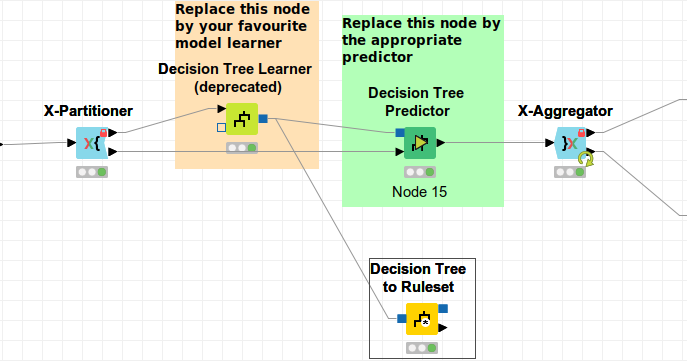
\includegraphics[scale=0.5]{flow-c45-p.png}  %el parámetro scale permite agrandar o achicar la imagen. En el nombre de archivo puede especificar directorios
	\caption{Flow del C4.5 KNIME} 
	\label{fig:flowc4.5}
\end{figure}



Para configurar el árbol de decisión, decido utilizar el índice de Gini como medida de cualidad y no hacer poda. Establezco, además, 4 hebras.

\begin{figure}[H] %con el [H] le obligamos a situar aquí la figura
	\centering
	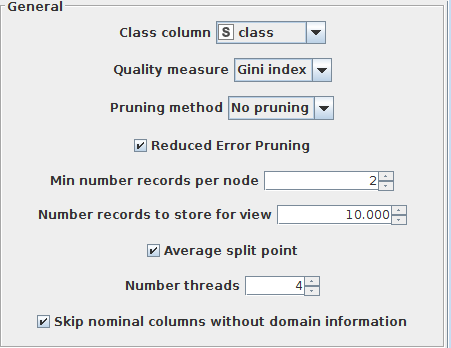
\includegraphics[scale=0.5]{confc45-p.png}  %el parámetro scale permite agrandar o achicar la imagen. En el nombre de archivo puede especificar directorios
	\caption{Configuración del Learner C4.5 KNIME} 
	\label{fig:confc45-p}
\end{figure}

Los resultados obtenidos son:

\begin{table}[H]
	\centering
	\begin{tabular}{|l|l|l|l|l|l|l|}
		\hline
		Row ID      & TPR   & TNR   & AUC   & Valor-F1 & G-mean   & Accuracy \\ \hline
		no\_popular & 0.823 & 0.275 &       & 0.809    & 0.475736 &          \\ \hline
		popular     & 0.275 & 0.823 & 0.556 & 0.292    & 0.475736 &          \\ \hline
		Overall     &       &       &       &          &          & 0.7      \\ \hline
	\end{tabular}
	\caption{Resultados de la ejecución del C4.5}
	\label{tab:c45}
\end{table}

y su curva ROC:

\begin{figure}[H] %con el [H] le obligamos a situar aquí la figura
	\centering
	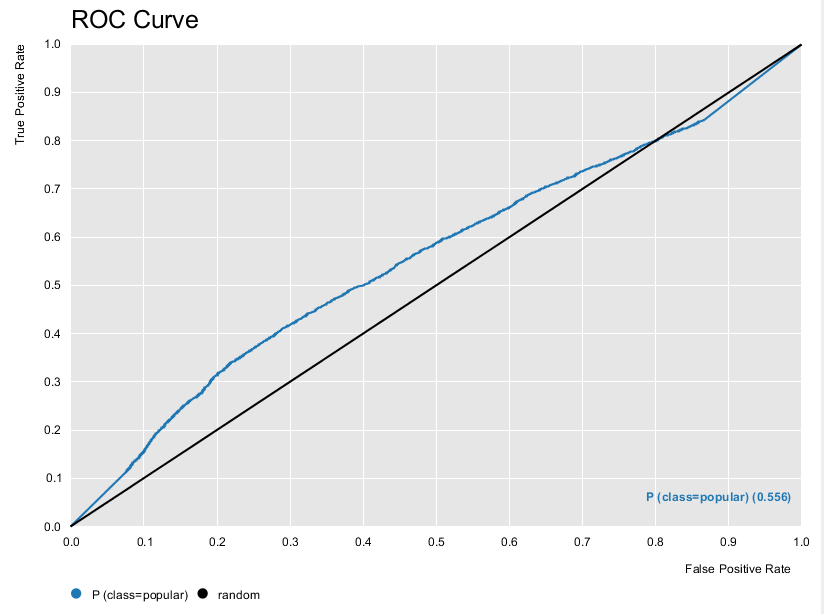
\includegraphics[scale=0.385]{roc-c45-p.png}  %el parámetro scale permite agrandar o achicar la imagen. En el nombre de archivo puede especificar directorios
	\caption{Curva ROC C4.5 KNIME} 
	\label{fig:rocc45-p}
\end{figure}

La complejidad del modelo es el número de hojas. A través de un \textit{Decision Tree to Ruleset}, contando el número de filas, veo que tiene 2551 reglas (hojas).

\subsection{Random Forest}

\begin{figure}[H] %con el [H] le obligamos a situar aquí la figura
	\centering
	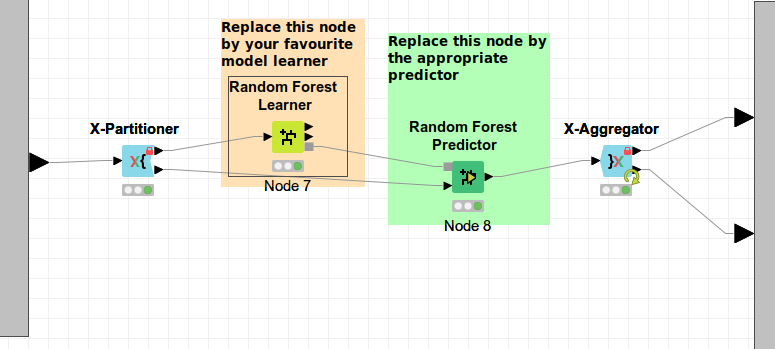
\includegraphics[scale=0.4]{flow-rf-p.png}  %el parámetro scale permite agrandar o achicar la imagen. En el nombre de archivo puede especificar directorios
	\caption{Flow del Random Forest} 
	\label{fig:flow-rf}
\end{figure}



A través de este algoritmo se genera un modelo con 100 clasificadores sobre 51 atributos. Los resultados obtenidos con este clasificador son:


\begin{table}[H]
	\centering
	\begin{tabular}{|l|l|l|l|l|l|l|}
		\hline
		Row ID      & TPR   & TNR   & AUC   & Valor-F1 & G-mean    & Accuracy \\ \hline
		no\_popular & 0.983 & 0.072 &       & 0.873    & 0.2660375 &          \\ \hline
		popular     & 0.072 & 0.983 & 0.699 & 0.127    & 0.2660375 &          \\ \hline
		Overall     &       &       &       &          &           & 0.778    \\ \hline
	\end{tabular}
	\caption{Resultados de la ejecución del Random Forest}
	\label{tab:rf}
\end{table}

y su curva ROC:

\begin{figure}[H] %con el [H] le obligamos a situar aquí la figura
	\centering
	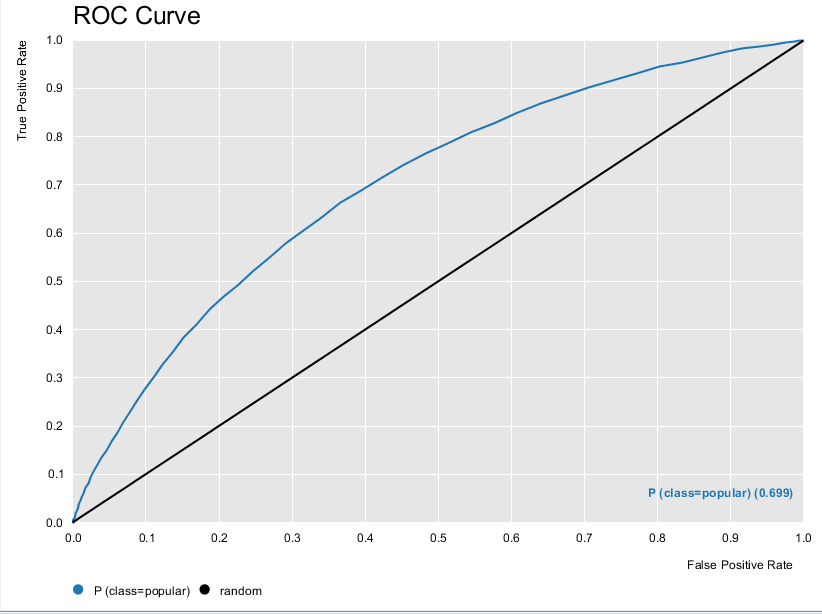
\includegraphics[scale=0.335]{roc-rf-p.png}  %el parámetro scale permite agrandar o achicar la imagen. En el nombre de archivo puede especificar directorios
	\caption{Curva ROC Random Forest} 
	\label{fig:rocrf-p}
\end{figure}

\subsection{KNN}

\begin{figure}[H] %con el [H] le obligamos a situar aquí la figura
	\centering
	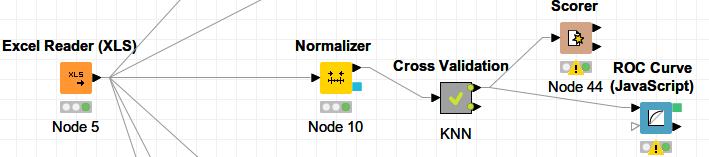
\includegraphics[scale=0.4]{flow-knn-p.png}  %el parámetro scale permite agrandar o achicar la imagen. En el nombre de archivo puede especificar directorios
	\caption{Flow del KNN} 
	\label{fig:flow-knn}
\end{figure}

Para emplear KNN es necesario normalizar los datos previamente, ya que es un algoritmo basado en distancias (normalización min-max [0,1]). Además, en su configuración establezco 3 como el número de vecinos.

\begin{figure}[H] %con el [H] le obligamos a situar aquí la figura
	\centering
	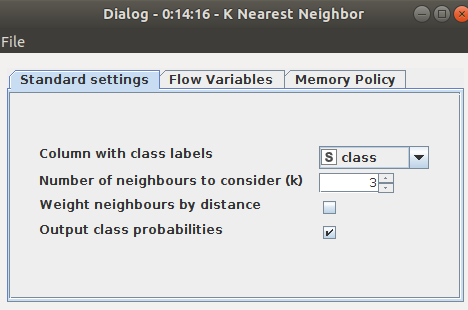
\includegraphics[scale=0.4]{conf-knn-p.png}  %el parámetro scale permite agrandar o achicar la imagen. En el nombre de archivo puede especificar directorios
	\caption{Configuración del KNN} 
	\label{fig:conf-knn-p}
\end{figure}

Los resultados obtenidos son:

\begin{table}[H]
	\centering
	\begin{tabular}{|l|l|l|l|l|l|l|}
		\hline
		Row ID      & TPR   & TNR   & AUC   & Valor-F1 & G-mean    & Accuracy \\ \hline
		no\_popular & 0.881 & 0.209 &       & 0.835    & 0.4291025 &          \\ \hline
		popular     & 0.209 & 0.881 & 0.547 & 0.258    & 0.4291025 &          \\ \hline
		Overall     &       &       &       &          &           & 0.731    \\ \hline
	\end{tabular}
	\caption{Resultados de la ejecución del KNN}
	\label{tab:knn}
\end{table}

y su curva ROC:

\begin{figure}[H] %con el [H] le obligamos a situar aquí la figura
	\centering
	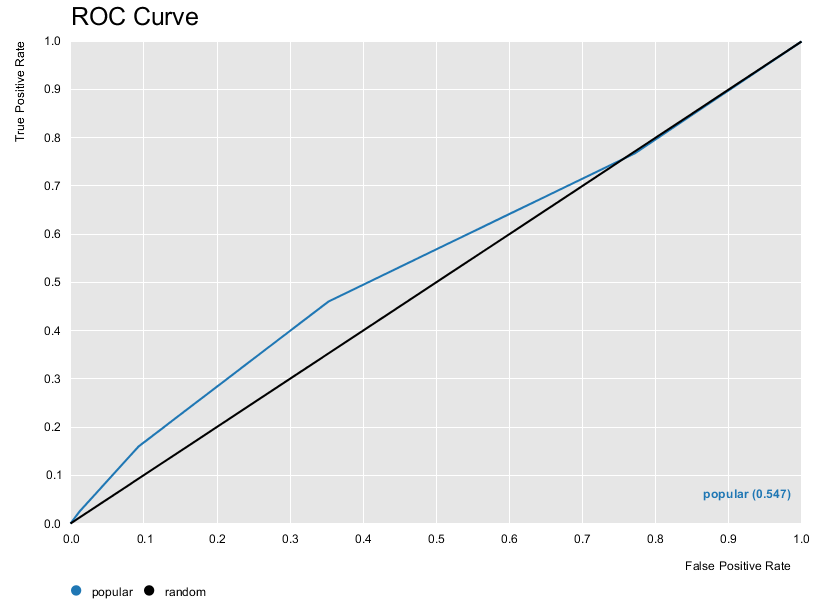
\includegraphics[scale=0.38]{roc-knn-p.png}  %el parámetro scale permite agrandar o achicar la imagen. En el nombre de archivo puede especificar directorios
	\caption{Curva ROC KNN} 
	\label{fig:rocknn-p}
\end{figure}

\subsection{Naïve-Bayes}

\begin{figure}[H] %con el [H] le obligamos a situar aquí la figura
	\centering
	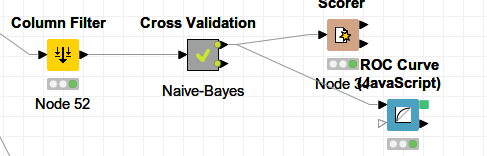
\includegraphics[scale=0.4]{flow-nb-p.png}  %el parámetro scale permite agrandar o achicar la imagen. En el nombre de archivo puede especificar directorios
	\caption{Flow del Naïve-Bayes} 
	\label{fig:flow-nb}
\end{figure}

A través del Column Filter elimino la columna \textit{weekday} por ser categórica. Además, defino como probabilidad por defecto en el Learner 0 y 20 como el máximo de variables nominales únicas por cada atributo. Por último, ignoro los valores perdidos.

Como resultados, se obtienen:

\begin{table}[H]
	\centering
	\begin{tabular}{|l|l|l|l|l|l|l|}
		\hline
		Row ID      & TPR   & TNR   & AUC   & Valor-F1 & G-mean   & Accuracy \\ \hline
		no\_popular & 0.524 & 0.698 &       & 0.65     & 0.604774 &          \\ \hline
		popular     & 0.698 & 0.524 & 0.643 & 0.418    & 0.604774 &          \\ \hline
		Overall     &       &       &       &          &          & 0.563    \\ \hline
	\end{tabular}
	\caption{Resultados de la ejecución del Naive-Bayes}
	\label{tab:nb}
\end{table}

y como curva ROC:


\begin{figure}[H] %con el [H] le obligamos a situar aquí la figura
	\centering
	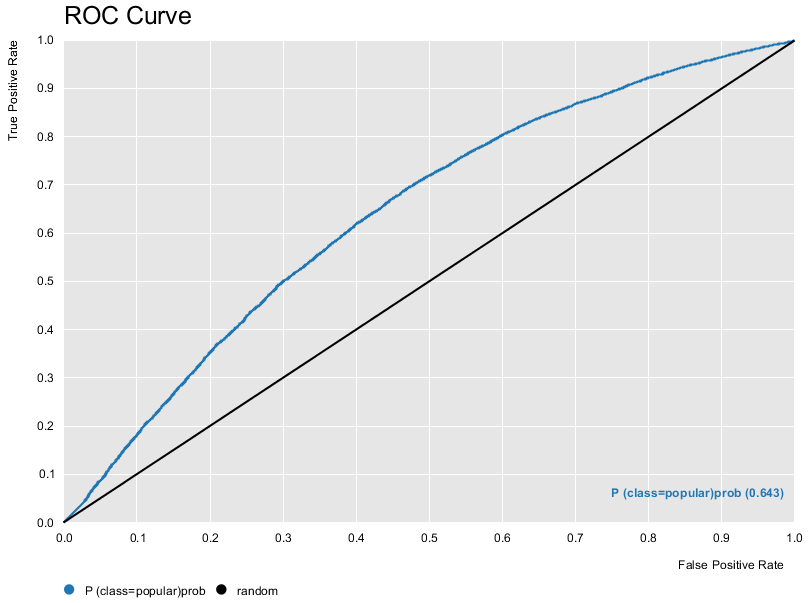
\includegraphics[scale=0.38]{roc-nb-p.png}  %el parámetro scale permite agrandar o achicar la imagen. En el nombre de archivo puede especificar directorios
	\caption{Curva ROC Naïve-Bayes} 
	\label{fig:rocknb-p}
\end{figure}

\subsection{SVM}

\begin{figure}[H] %con el [H] le obligamos a situar aquí la figura
	\centering
	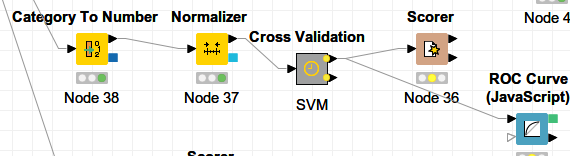
\includegraphics[scale=0.4]{flow-svm-p.png}  %el parámetro scale permite agrandar o achicar la imagen. En el nombre de archivo puede especificar directorios
	\caption{Flow del SVM} 
	\label{fig:flow-svm}
\end{figure}

Como requiere que los datos sean linealmente separables, es necesario eliminar las variables categóricas (Category to Number en \textit{weekday}). Además, también necesita normalización. Establezco la siguiente configuración:

\begin{figure}[H] %con el [H] le obligamos a situar aquí la figura
	\centering
	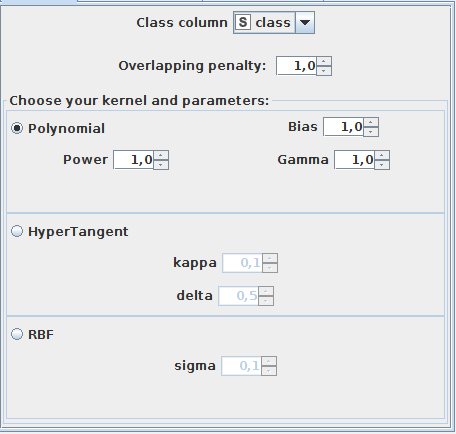
\includegraphics[scale=0.4]{conf-svm-p.png}  %el parámetro scale permite agrandar o achicar la imagen. En el nombre de archivo puede especificar directorios
	\caption{Configuración del SVM} 
	\label{fig:conf-svm}
\end{figure}

Se puede observar que escojo un kernel polinomial con valores por defecto. Con esa configuración, la ejecución del algoritmo es totalmente inabordable en tiempo (más de 5 horas y sin resultado, llegando incluso a colgar KNIME). Por eso, uno de los objetivos que me marco en esta práctica es preprocesar los datos y reducir su dimensionalidad con técnicas de estadística multivariante para llegar a extraer, al menos, algunos resultados en clasificación, preferentemente competitivos.

\subsection{Gradient Boosted}

\begin{figure}[H] %con el [H] le obligamos a situar aquí la figura
	\centering
	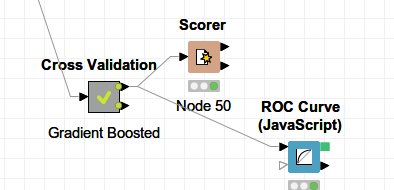
\includegraphics[scale=0.4]{flow-gb-p.png}  %el parámetro scale permite agrandar o achicar la imagen. En el nombre de archivo puede especificar directorios
	\caption{Flow del Gradient Boost} 
	\label{fig:flow-gb}
\end{figure}

Establezco la siguiente configuración en dicho árbol:

\begin{figure}[H] %con el [H] le obligamos a situar aquí la figura
	\centering
	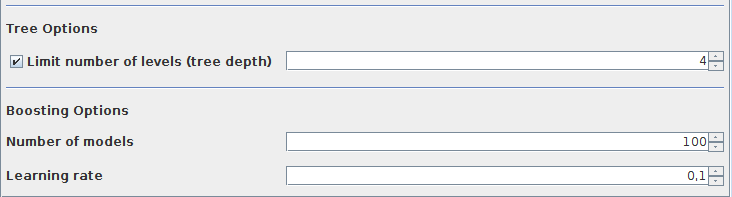
\includegraphics[scale=0.4]{conf-gb-p.png}  %el parámetro scale permite agrandar o achicar la imagen. En el nombre de archivo puede especificar directorios
	\caption{Configuración del Gradient Boosted} 
	\label{fig:conf-gb}
\end{figure}

Los resultados obtenidos son:

\begin{table}[H]
	\centering
	\begin{tabular}{|l|l|l|l|l|l|l|}
		\hline
		Row ID      & TPR   & TNR   & AUC   & Valor-F1 & G-mean   & Accuracy \\ \hline
		no\_popular & 0.977 & 0.092 &       & 0.872    & 0.299806 &          \\ \hline
		popular     & 0.092 & 0.977 & 0.716 & 0.157    & 0.299806 &          \\ \hline
		Overall     &       &       &       &          &          & 0.778    \\ \hline
	\end{tabular}
	\caption{Resultados de la ejecución del Gradient Boosting}
	\label{tab:gb}
\end{table}

Su curva ROC es:

\begin{figure}[H] %con el [H] le obligamos a situar aquí la figura
	\centering
	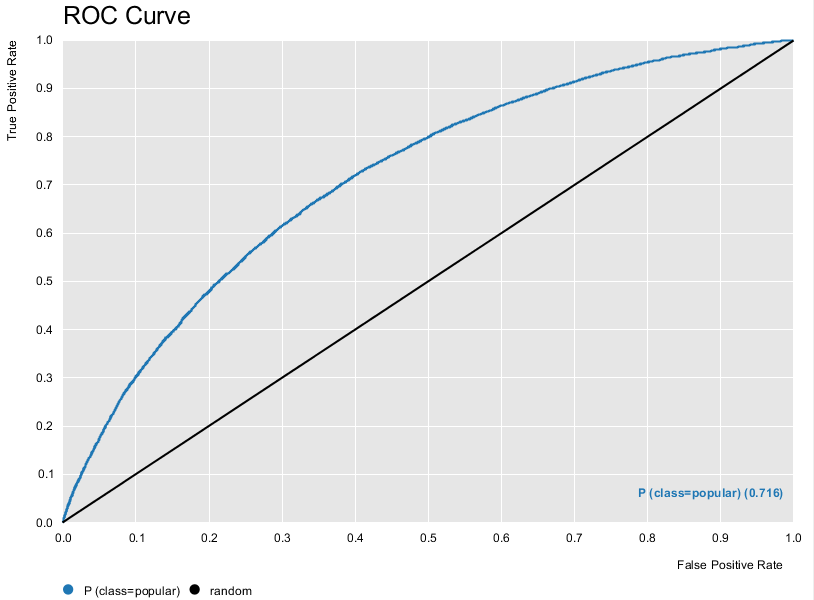
\includegraphics[scale=0.38]{roc-gb-p.png}  %el parámetro scale permite agrandar o achicar la imagen. En el nombre de archivo puede especificar directorios
	\caption{Curva ROC Gradient Boosted} 
	\label{fig:rocgb-p}
\end{figure}

\subsection{RProp MLP}

\begin{figure}[H] %con el [H] le obligamos a situar aquí la figura
	\centering
	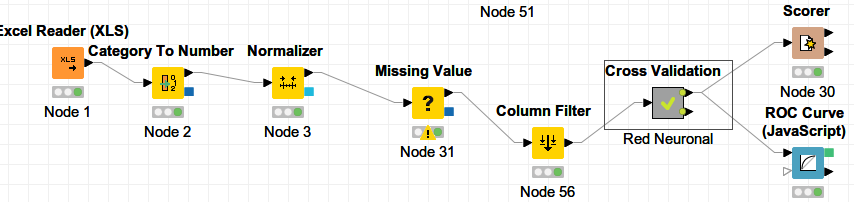
\includegraphics[scale=0.4]{flow-rn-p.png}  %el parámetro scale permite agrandar o achicar la imagen. En el nombre de archivo puede especificar directorios
	\caption{Flow de la red neuronal MLP} 
	\label{fig:flow-rn-p}
\end{figure}

Por definición, las redes neuronales necesitan trabajar con valores numéricos y normalizados. Además, requieren un tratamiento de valores perdidos (en este caso, se eliminan las filas con valores perdidos).\\

Por motivos de eficiencia, he establecido 2 como el máximo número de iteraciones, 2 el número de capas ocultas y 10 el número de neuronas ocultas por capa (en casos mayores sobrepasaba la capacidad del Heap). 

\begin{figure}[H] %con el [H] le obligamos a situar aquí la figura
	\centering
	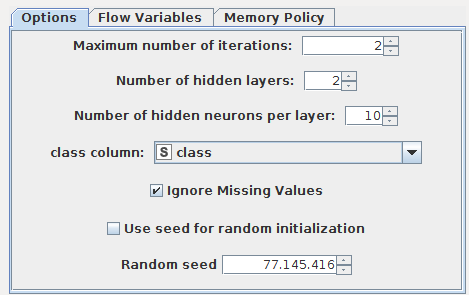
\includegraphics[scale=0.33]{conf-rn-p.png}  %el parámetro scale permite agrandar o achicar la imagen. En el nombre de archivo puede especificar directorios
	\caption{Configuración de la red neuronal} 
	\label{fig:conf-rn}
\end{figure}

Los resultados obtenidos son:

\begin{table}[H]
	\centering
	\begin{tabular}{|l|l|l|l|l|l|l|}
		\hline
		Row ID      & TPR & TNR & AUC   & Valor-F1 & G-mean & Accuracy \\ \hline
		no\_popular & 1   & 0   &       & 0.874    & 0      &          \\ \hline
		popular     & 0   & 1   & 0.496 & 0        & 0      &          \\ \hline
		Overall     &     &     &       &          &        & 0.776    \\ \hline
	\end{tabular}
	\caption{Resultados de la ejecución del MLP}
	\label{tab:mlp}
\end{table}

y su curva ROC es

\begin{figure}[H] %con el [H] le obligamos a situar aquí la figura
	\centering
	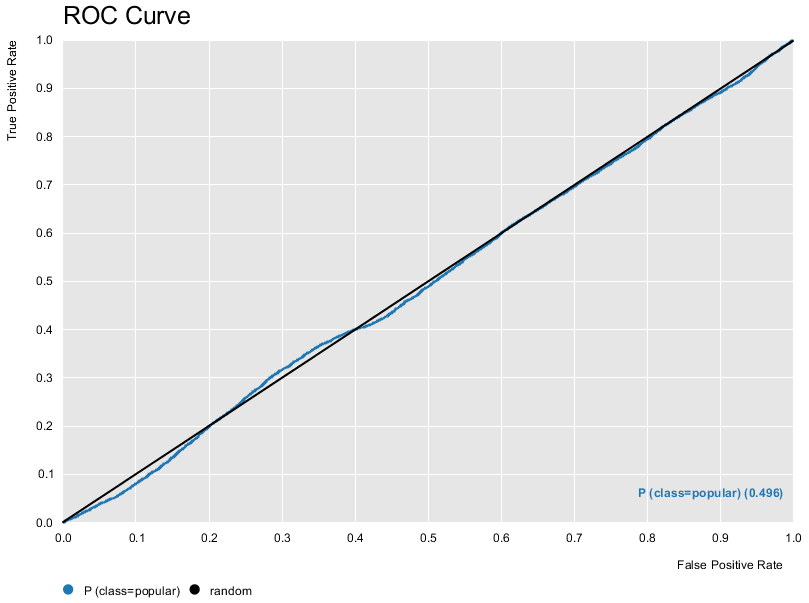
\includegraphics[scale=0.36]{roc-rn-p.png}  %el parámetro scale permite agrandar o achicar la imagen. En el nombre de archivo puede especificar directorios
	\caption{Curva ROC de la red neuronal} 
	\label{fig:rocrn-p}
\end{figure}

%----------------------------------------------------------------------------------------


%----------------------------------------------------------------------------------------
%	Análisis de resultados
%----------------------------------------------------------------------------------------

\section{Análisis de resultados}

Para comparar los resultados, aúno en un mismo plano cartesiano todas las curvas ROC (a excepción del MLP, ya que se le han eliminado muchas instancias con valores perdidos y no es comparable con los demás en la misma gráfica. Aún así, se obtienen resultados muy pobres). He aquí el resultado:

\begin{figure}[H] %con el [H] le obligamos a situar aquí la figura
	\centering
	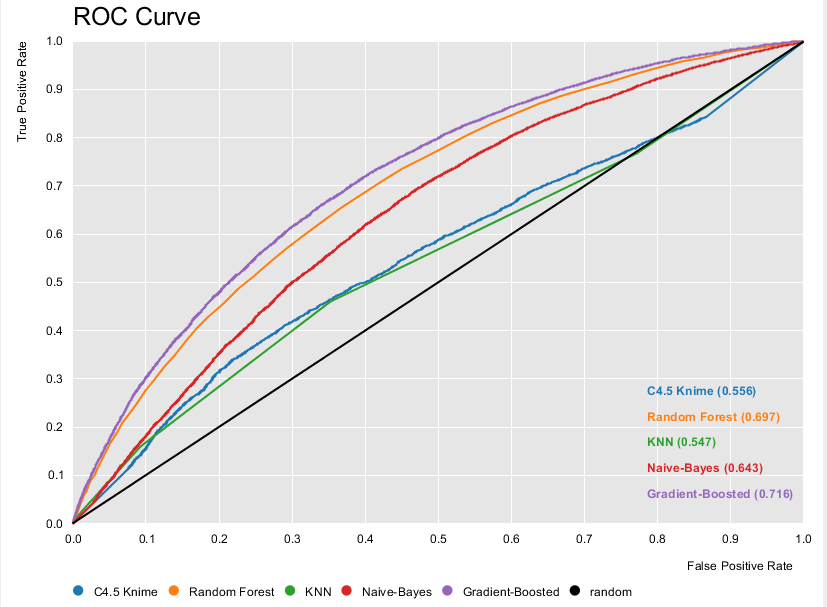
\includegraphics[scale=0.38]{roc-all-p.png}  %el parámetro scale permite agrandar o achicar la imagen. En el nombre de archivo puede especificar directorios
	\caption{Curva ROC de todos los clasificadores (excepto SVM y MLP)} 
	\label{fig:rocall-p}
\end{figure}

Como se puede apreciar, los mejores resultados vienen dados por Gradient-Boosting (GBT), seguidos de Random Forest, Naive-Bayes, C4.5 KNIME y KNN. En las últimas posiciones se encontrarían MLP (con un AUC por debajo de 0.5) y SVM, que ni siquiera llega a ejecutarse. Por tanto, los ensamble parece ir mejor que los demás. De hecho, según podemos leer en \cite{friedman}, GBT son especialmente útiles para problemas donde se presenta gran desbalanceo, ya que engrandece el impacto de la clase positiva. Además, cabe esperar mejora debido a la sensibilidad del algoritmo al ruido. Sería interesante estudiar el sobreajuste del modelo. Por su parte, Random Forest es robusto al ruido y a los valores perdidos. El resto sufren el desbalanceo del conjunto de datos, lo que penaliza muchísimo el resultado. 


%------------------------------------------------

%----------------------------------------------------------------------------------------
%	Configuración de algoritmos
%----------------------------------------------------------------------------------------

\section{Configuración de algoritmos}


Mi empeño en la presente sección será modificar ciertos parámetros de los algoritmos. Para ello, utilizo un nodo llamado Paremeter Optimization Loop Start/Paremeter Optimization Loop End (descrito en \cite{param-opt}), donde se definen los parámetros que se quieren observar y se itera sobre todos sus posibles valores. Finalmente, se configura para que se maximice el \textit{accuracy}. Por cuestión de eficiencia, utilizo en cada flujo un particionamiento con 80\% para entrenamiento y 20\% para test.

\subsection{C4.5 KNIME}

\begin{figure}[H] %con el [H] le obligamos a situar aquí la figura
	\centering
	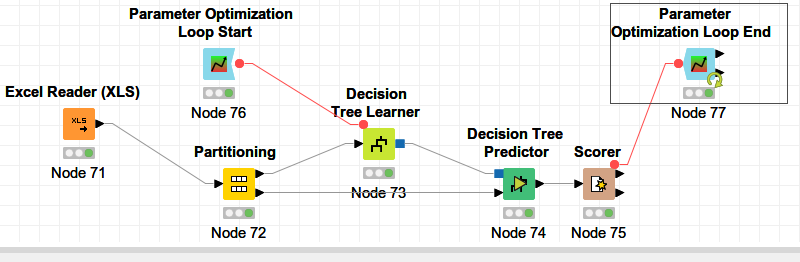
\includegraphics[scale=0.38]{flow-param-c45.png}  %el parámetro scale permite agrandar o achicar la imagen. En el nombre de archivo puede especificar directorios
	\caption{Flow de configuración de parámetros C4.5} 
	\label{fig:conf-c45}
\end{figure}


\underline{\textbf{Parametros obtenidos:}} \\
\begin{itemize}
	\item Quality measure: Gain ratio
	\item Pruning method: MDL
	\item Min number records per node: 4 
	\item Number records to store for view: 8000
\end{itemize}
\textbf{Accuracy:} 0.775 (Respecto 0.7 anterior)

Probando estos datos en mi flow con validación cruzada, AUC sube a 0.62 (0.556 antes) y se reduce a 14 reglas (hojas), por lo que la ganancia es enorme.

\subsection{Random Forest}

\begin{figure}[H] %con el [H] le obligamos a situar aquí la figura
	\centering
	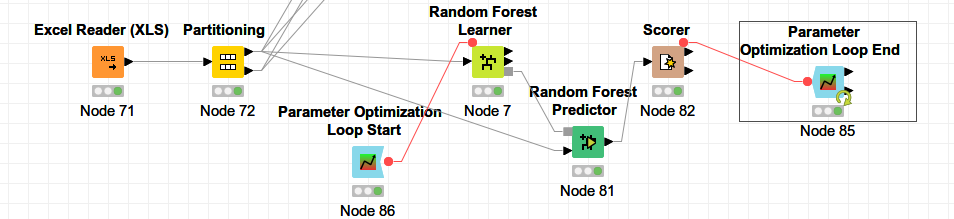
\includegraphics[scale=0.38]{flow-param-rf.png}  %el parámetro scale permite agrandar o achicar la imagen. En el nombre de archivo puede especificar directorios
	\caption{Flow de configuración de parámetros Random Forest} 
	\label{fig:conf-rf}
\end{figure}

Configurando el número de modelos a 137, la clasificación tiene un 100\% de \textit{accuracy}. Soy excéptico con este resultado, pudiendo haber alguna anomalía en la configuración. No obstante, muestro los resultados:


\begin{figure}[H] %con el [H] le obligamos a situar aquí la figura
	\centering
	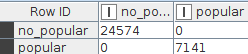
\includegraphics[scale=0.8]{acc-rf-param.png}  %el parámetro scale permite agrandar o achicar la imagen. En el nombre de archivo puede especificar directorios
	\caption{Resultados tras la configuración de parámetros Random Forest (137 modelos)} 
	\label{fig:acc-param-rf}
\end{figure}


\subsection{KNN}

\begin{figure}[H] %con el [H] le obligamos a situar aquí la figura
	\centering
	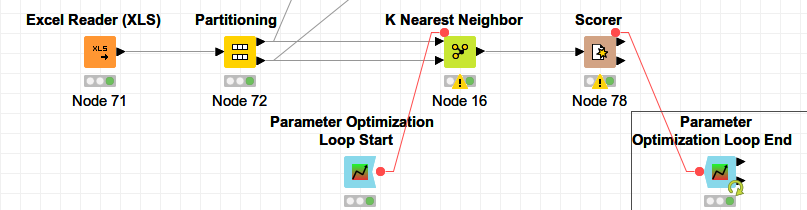
\includegraphics[scale=0.38]{flow-param-knn.png}  %el parámetro scale permite agrandar o achicar la imagen. En el nombre de archivo puede especificar directorios
	\caption{Flow de configuración de parámetros KNN} 
	\label{fig:conf-knn}
\end{figure}

\underline{\textbf{Parametros obtenidos:}} \\
\begin{itemize}
	\item k: 10
\end{itemize}

\textbf{Accuracy:} 0.769 (Respecto 0.731 anterior)
Probando este parámetro en mi flow anterior, AUC aumenta hasta 0.572, una leve mejora.

\subsection{Naïve-Bayes}

\begin{figure}[H] %con el [H] le obligamos a situar aquí la figura
	\centering
	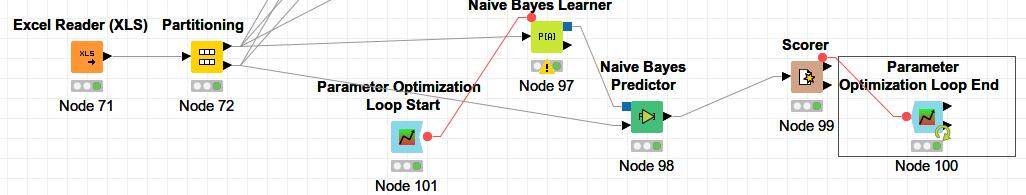
\includegraphics[scale=0.38]{flow-param-nb.png}  %el parámetro scale permite agrandar o achicar la imagen. En el nombre de archivo puede especificar directorios
	\caption{Flow de configuración de parámetros Naïve-Bayes} 
	\label{fig:conf-nb}
\end{figure}

\underline{\textbf{Parametros obtenidos:}} \\
\begin{itemize}
	\item Default probability: 0.901
	\item Maximum number of unique nominal values per attribute: 18
\end{itemize}

\textbf{Accuracy:} 0.775 (Respecto 0.563 anterior)
Sin embargo, al reflejar dichos cambios en la validación cruzada, se obtienen los mismos resultados que antes.


%----------------------------------------------------------------------------------------
%	Procesando datos
%----------------------------------------------------------------------------------------

\section{Procesado de datos}

Nuestro próximo objetivo será preprocesar los datos para obtener un mejor comportamiento en los algoritmos de clasificación. Para ello,  me baso en el artículo \cite{preprocessing} siguiendo el orden que proponen, es decir, primero se elimina el ruido y los valores perdidos, luego se reduce la dimensionalidad y por último se balancea el dataset. A pesar de no ser un procedimiento con éxito asegurado, es lógico hacerlo así, ya que si no elimináramos el ruido al principio, estaríamos estudiando las relaciones entre variables con datos probablemente erróneos. Además, en el balanceo yo propongo utilizar SMOTE, luego generaríamos de forma sintética datos basados en otros con ruido. Veamos el flujo de trabajo y sus distintos metadonos.

\begin{figure}[H] %con el [H] le obligamos a situar aquí la figura
	\centering
	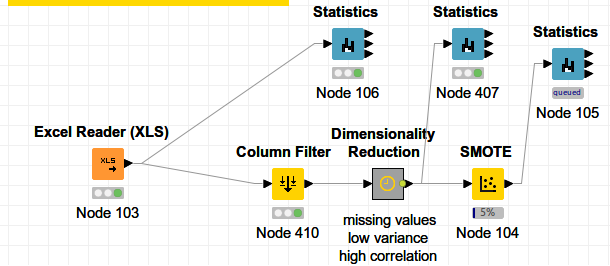
\includegraphics[scale=0.6]{flow-prep.png}  %el parámetro scale permite agrandar o achicar la imagen. En el nombre de archivo puede especificar directorios
	\caption{Flow de preprocesamiento} 
	\label{fig:flow-prep}
\end{figure}


\subsection{Reducción de la dimensionalidad}

Es crucial tratar de reducir la dimensionalidad en pos de la eficiencia de los algoritmos y también de sus resultados, ya que se favorecería la interpretabilidad de los modelos. Para ello, basándome en los apartados \textit{Imperfect Data} y \textit{Data Reduction} de \cite{preprocessing}, \cite{dr2} y en \cite{dr}, defino el metanodo \textit{Dimensionality Reduction}:

\begin{figure}[H] %con el [H] le obligamos a situar aquí la figura
	\centering
	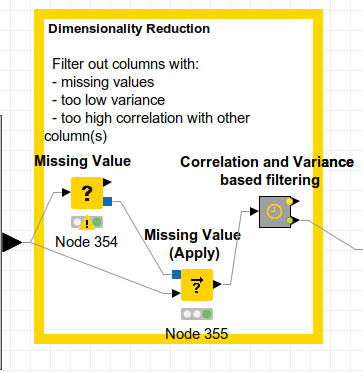
\includegraphics[scale=0.6]{flow-dr.png}  %el parámetro scale permite agrandar o achicar la imagen. En el nombre de archivo puede especificar directorios
	\caption{Flow del metadonodo Dimensionality Reduction} 
	\label{fig:flow-dr}
\end{figure}

Como se puede ver, hago un tratamiento de valores perdidos, low variance y high correlation.

\subsubsection{Valores perdidos}

En lo que se refiere a valores perdidos, el tratamiento en mi caso es sencillo: simplemente elimino la fila que contenga valores perdidos de cualquier tipo. El motivo es doble. En primer lugar, podría utilizar de nuevo machine learning para inferir e imputar valores perdidos, pero el coste computacional sería tremendo dado que el 25\% de las instancias tienen valores perdidos. Por otra parte, al quitar ese 25\%, ya hago una selección de instancias. Es cierto que no utilizo ninguna técnica de estadística multivariante para seleccionar esas instancias, pero en la literatura encontramos que a menudo es útil eliminar directamente las instancias.

\subsubsection{Correlación y varianza de las variables (Seleción de características)}

\begin{figure}[H] %con el [H] le obligamos a situar aquí la figura
	\centering
	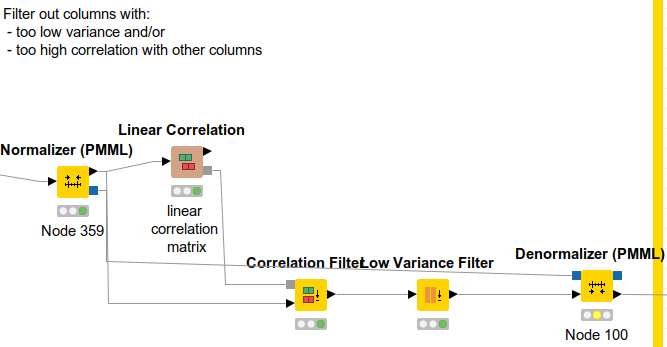
\includegraphics[scale=0.5]{flow-cr.png}  %el parámetro scale permite agrandar o achicar la imagen. En el nombre de archivo puede especificar directorios
	\caption{Flow del metadonodo Correlation and Variation} 
	\label{fig:flow-cv}
\end{figure}

Tras una normalización min-max (según el estándar PMML), evalúo un modelo de correlación lineal (\cite{cf}) para así eliminar aquellas características con una varianza baja. Expongo las distintas configuraciones:

\textbf{Linear Correlation:} Todas las variables son incluidas excepto la clase.\\
\textbf{Correlation filter:} Establezco \textit{Correlation Threshold:0.72}, por lo que se reducen a 37 las columnas que quedan. \\
\textbf{Variance Filter:} Variance upper bound = 0.05.

Tras los anterior, el dataset se ha reducido a 30567 filas y 13 columnas.



\subsection{Desbalanceo del conjunto de datos}

El conjunto de datos está muy desbalanceado. Desde un punto de vista lógico, lo normal es que así sea, ya que la mayoría de las publicaciones en la web en forma de noticias (no olvidemos que este es nuestro problema) no se hacen virales. Sin embargo, desde el punto de vista de la ciencia de datos, esto supone un gran perjuicio.

\begin{figure}[H] %con el [H] le obligamos a situar aquí la figura
	\centering
	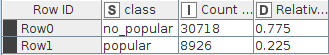
\includegraphics[scale=0.6]{unbalanced-data.png}  %el parámetro scale permite agrandar o achicar la imagen. En el nombre de archivo puede especificar directorios
	\caption{Tabla de datos que muestra el desbalanceo entre las dos clases} 
	\label{fig:unb-data}
\end{figure}

\begin{figure}[H] %con el [H] le obligamos a situar aquí la figura
	\centering
	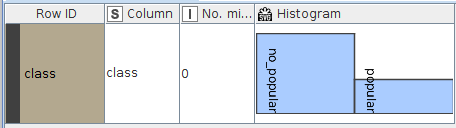
\includegraphics[scale=0.6]{hist-unb-data.png}  %el parámetro scale permite agrandar o achicar la imagen. En el nombre de archivo puede especificar directorios
	\caption{Histograma de los datos sin tratar} 
	\label{fig:hist-unb-data}
\end{figure}

Para tratar este problema, utilizo el algoritmo \textit{SMOTE}, estudiado en la teoría de esta asignatura (\cite{smote}). Lo configuro con 7 vecinos más cercanos para que genere instancias de datos con la clase minoritaria. Ahora que la reducción de datos ha sido completada, la ejecución de SMOTE es mucho más ligera. Este es el resultado:

\begin{figure}[H] %con el [H] le obligamos a situar aquí la figura
	\centering
	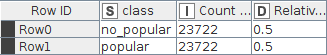
\includegraphics[scale=0.6]{b-dat.png}  %el parámetro scale permite agrandar o achicar la imagen. En el nombre de archivo puede especificar directorios
	\caption{Tabla de datos tras Smote} 
	\label{fig:hist-b-data}
\end{figure}

\newpage

%----------------------------------------------------------------------------------------
%	Interpretación de los resultados
%----------------------------------------------------------------------------------------

\section{Interpretación de los resultados}

Tras el preprocesado de datos, aplicamos dicho metanodo a nuestra estructura de Data Mining en pos de comprobar si han mejorado los resultados. Para ello, haré otro repaso por todos los algoritmos mediante una tabla resumen comparativa (datos con \_np son previos al preprocesamiento, \_p posteriores al preprocesamiento) para finalmente aunarlas en una gran tabla final con los resultados de los algoritmos. Se tratará finalmente de especificar qué características son determinantes (o más importantes) en la inferencia de la popularidad de la noticia y que algoritmos funcionan mejor.


\begin{figure}[H] %con el [H] le obligamos a situar aquí la figura
	\centering
	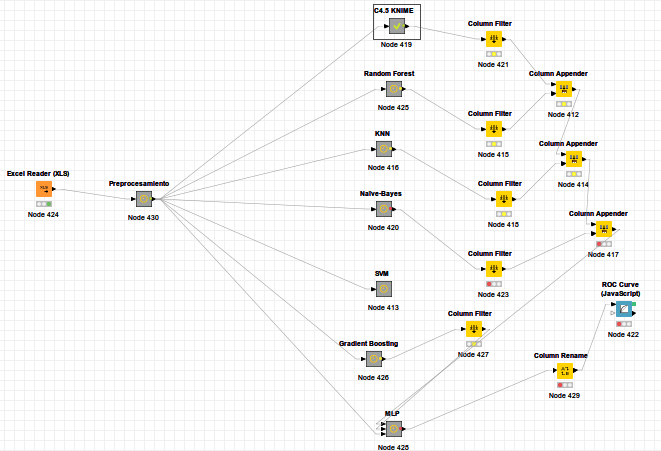
\includegraphics[scale=0.6]{flow-completo.png}  %el parámetro scale permite agrandar o achicar la imagen. En el nombre de archivo puede especificar directorios
	\caption{Flow de algoritmos con metanodo de preprocesado} 
	\label{fig:flow-completo}
\end{figure}

\subsection{C4.5 KNIME}


\begin{table}[H]
	\centering
	\begin{tabular}{|l|l|l|l|l|l|l|}
		\hline
		Row ID          & TPR   & TNR   & AUC   & Valor-F1 & G-mean   & Accuracy \\ \hline
		no\_popular\_np & 0.823 & 0.275 &       & 0.809    & 0.475736 &          \\ \hline
		no\_popular\_p  & 0.832 & 0.673 &       & 0.771    & 0.748288 &          \\ \hline
		popular\_np     & 0.275 & 0.823 & 0.556 & 0.292    & 0.475736 &          \\ \hline
		popular\_p      & 0.673 & 0.832 & 0.811 & 0.731    & 0.748288 &          \\ \hline
		Overall\_np     &       &       &       &          &          & 0.7      \\ \hline
		Overall\_p      &       &       &       &          &          & 0.753    \\ \hline
	\end{tabular}
	\caption{Comparación de resultados C4.5 KNIME}
	\label{tab:compc4.5}
\end{table}

Como se puede ver, se mejora ligeramente el accuracy pero AUC aumenta dramáticamente, como consecuencia, sobre todo, de haber balanceado el dataset. Por otra parte, hemos pasado de 2551 reglas a 613. Por tanto, el preprocesado está totalmente justificado.

\begin{figure}[H]
	\begin{subfigure}{.5\textwidth}
		\centering
		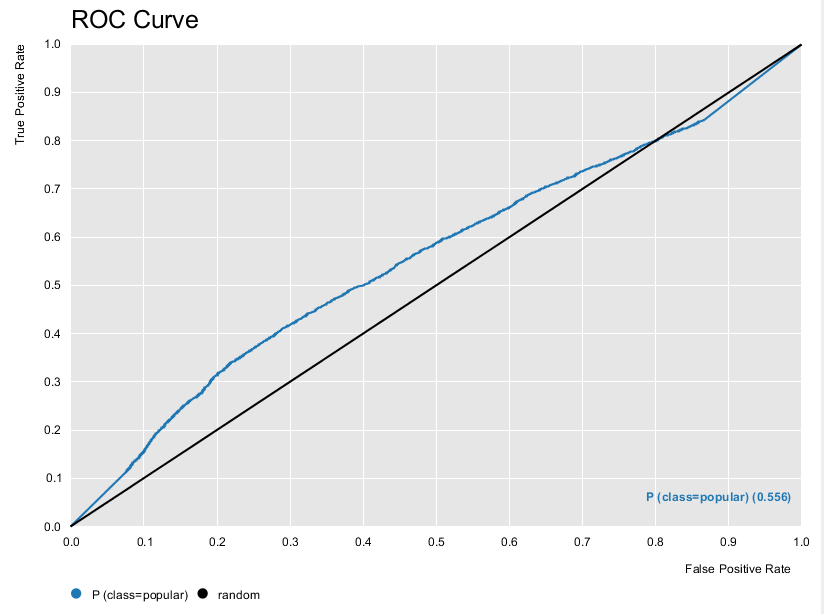
\includegraphics[width=.4\linewidth]{roc-c45-p.png}
		\caption{Curva ROC del C4.5 antes del preprocesamiento}
		\label{fig:rc45p}
	\end{subfigure}%
	\begin{subfigure}{.5\textwidth}
		\centering
		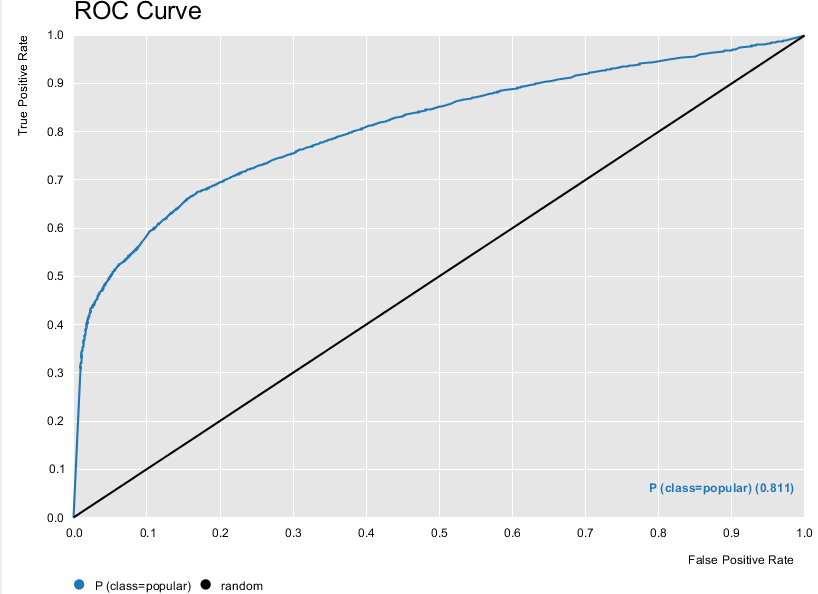
\includegraphics[width=.4\linewidth]{roc-c45.png}
		\caption{Curva ROC del C4.5 tras el preprocesamiento}
		\label{fig:rc45}
	\end{subfigure}
	\caption{Curvas ROC del C4.5}
	\label{fig:c4.5}
\end{figure}

\subsection{Random Forest}

\begin{table}[H]
	\centering
	\begin{tabular}{|l|l|l|l|l|l|l|}
		\hline
		Row ID          & TPR   & TNR   & AUC   & Valor-F1 & G-mean    & Accuracy \\ \hline
		no\_popular\_np & 0.983 & 0.072 &       & 0.873    & 0.2660375 &          \\ \hline
		no\_popular\_p  & 0.877 & 0.659 &       & 0.791    & 0.760225  &          \\ \hline
		popular\_np     & 0.072 & 0.983 & 0.699 & 0.127    & 0.2660375 &          \\ \hline
		popular\_p      & 0.659 & 0.877 & 0.854 & 0.731    & 0.760225  &          \\ \hline
		Overall\_np     &       &       &       &          &           & 0.778    \\ \hline
		Overall\_p      &       &       &       &          &           & 0.768    \\ \hline
	\end{tabular}
	\caption{Comparación de resultados Random Forest}
	\label{tab:comprf}
\end{table}

A pesar de que baja el accuracy en una centésima, AUC aumenta considerablemente teniendo unos buenos datos de clasificación.

\begin{figure}[H]
	\begin{subfigure}{.5\textwidth}
		\centering
		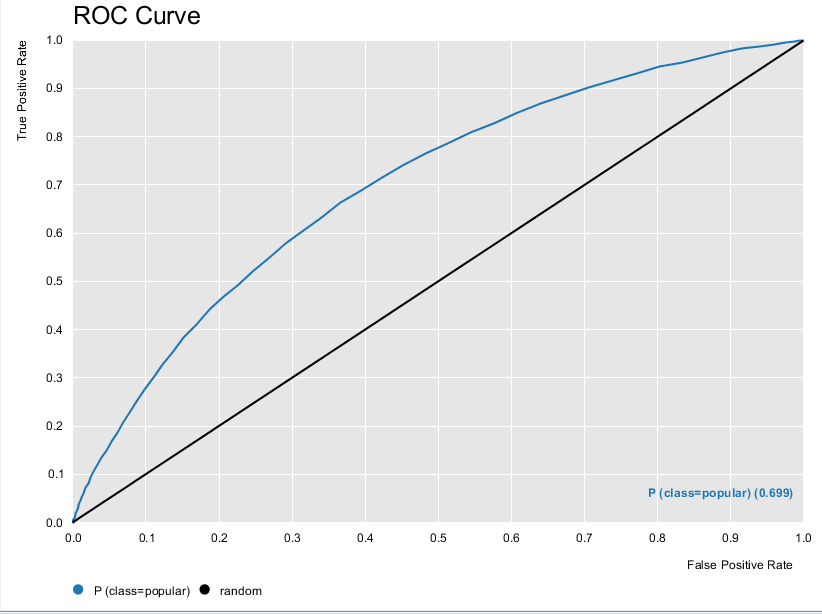
\includegraphics[width=.4\linewidth]{roc-rf-p.png}
		\caption{Curva ROC del Random Forest (previo)}
		\label{fig:rcrfp}
	\end{subfigure}%
	\begin{subfigure}{.5\textwidth}
		\centering
		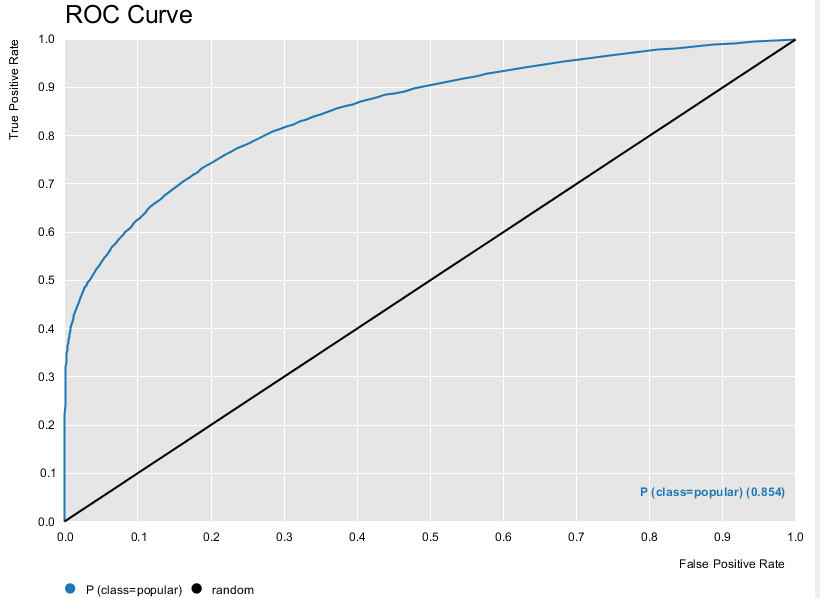
\includegraphics[width=.4\linewidth]{rc-rf.png}
		\caption{Curva ROC del Random Forest (posterior)}
		\label{fig:rcrf}
	\end{subfigure}
	\caption{Curvas ROC del Random Forest}
	\label{fig:rf}
\end{figure}

\subsection{KNN}

\begin{table}[H]
	\centering
	\begin{tabular}{|l|l|l|l|l|l|l|}
		\hline
		Row ID          & TPR   & TNR   & AUC   & Valor-F1 & G-mean    & Accuracy \\ \hline
		no\_popular\_np & 0.881 & 0.209 &       & 0.835    & 0.4291025 &          \\ \hline
		no\_popular\_p  & 0.737 & 0.686 &       & 0.718    & 0.711042  &          \\ \hline
		popular\_np     & 0.209 & 0.881 & 0.547 & 0.127    & 0.4291025 &          \\ \hline
		popular\_p      & 0.686 & 0.737 & 0.789 & 0.731    & 0.711042  &          \\ \hline
		Overall\_np     &       &       &       &          &           & 0.731    \\ \hline
		Overall\_p      &       &       &       &          &           & 0.711    \\ \hline
	\end{tabular}
	\caption{Comparación de resultados KNN}
	\label{tab:compknn}
\end{table}

Al igual que en los anteriores, el accuracy prácticamente se mantiene pero AUC aumenta considerablemente.

\begin{figure}[H]
	\begin{subfigure}{.5\textwidth}
		\centering
		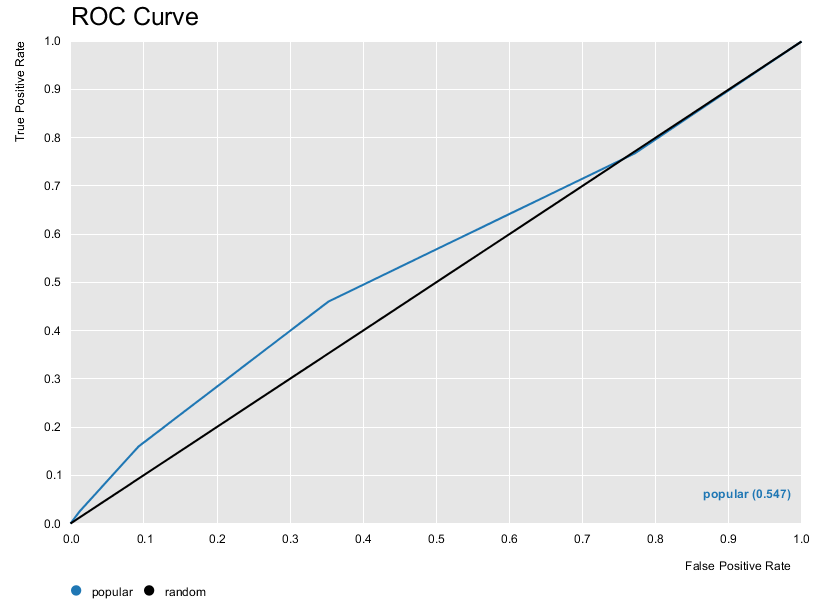
\includegraphics[width=.4\linewidth]{roc-knn-p.png}
		\caption{Curva ROC del KNN (previo)}
		\label{fig:rcknnp}
	\end{subfigure}%
	\begin{subfigure}{.5\textwidth}
		\centering
		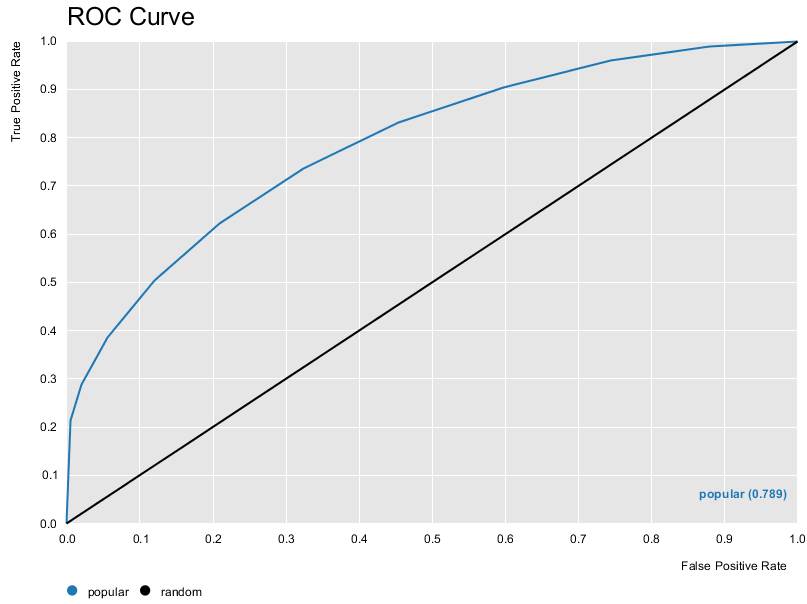
\includegraphics[width=.4\linewidth]{roc-knn.png}
		\caption{Curva ROC del KNN (posterior)}
		\label{fig:rcknn}
	\end{subfigure}
	\caption{Curvas ROC del KNN}
	\label{fig:bknn}
\end{figure}

\subsection{Naïve-Bayes}

\begin{table}[H]
	\centering
	\begin{tabular}{|l|l|l|l|l|l|l|}
		\hline
		Row ID          & TPR   & TNR   & AUC   & Valor-F1 & G-mean   & Accuracy \\ \hline
		no\_popular\_np & 0.524 & 0.698 &       & 0.65     & 0.604774 &          \\ \hline
		no\_popular\_p  & 0.802 & 0.436 &       & 0.678    & 0.591330 &          \\ \hline
		popular\_np     & 0.698 & 0.524 & 0.643 & 0.418    & 0.604774 &          \\ \hline
		popular\_p      & 0.436 & 0.802 & 0.674 & 0.533    & 0.591330 &          \\ \hline
		Overall\_np     &       &       &       &          &          & 0.563    \\ \hline
		Overall\_p      &       &       &       &          &          & 0.619    \\ \hline
	\end{tabular}
	\caption{Comparación de resultados Naïve-Bayes}
	\label{tab:compnb}
\end{table}

En este caso aumenta más el accuracy que AUC. Esto podría indicarnos que Naïve-Bayes necesitaría un preprocesamiento específico.

\begin{figure}[H]
	\begin{subfigure}{.5\textwidth}
		\centering
		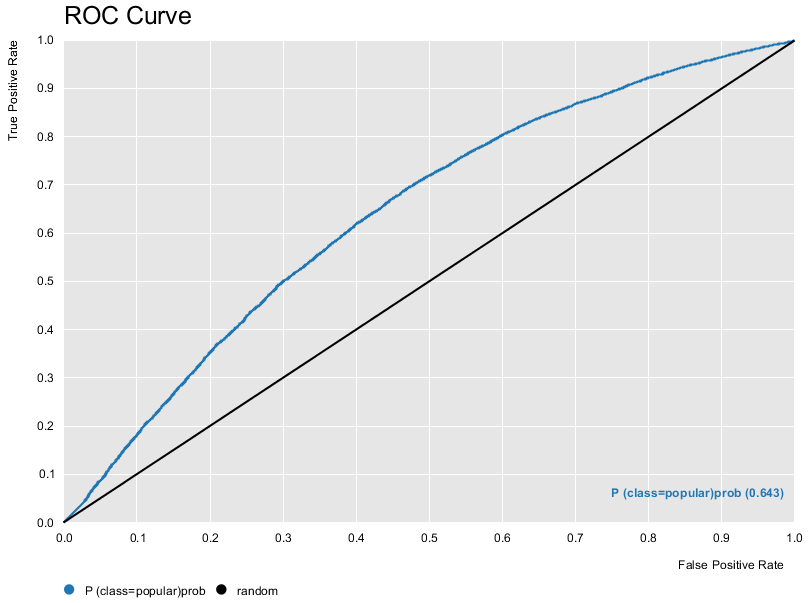
\includegraphics[width=.4\linewidth]{roc-nb-p.png}
		\caption{Curva ROC del N-B (previo)}
		\label{fig:rcnbp}
	\end{subfigure}%
	\begin{subfigure}{.5\textwidth}
		\centering
		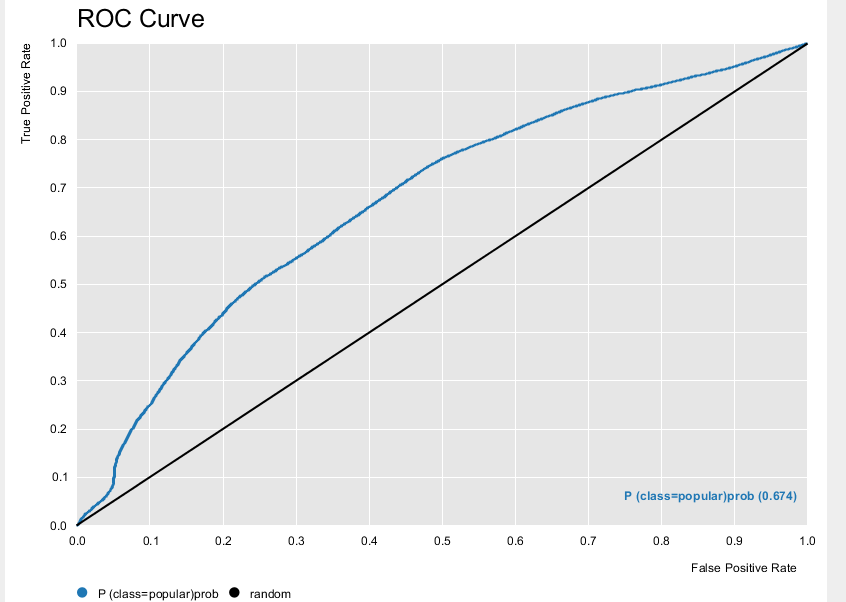
\includegraphics[width=.4\linewidth]{roc-nb.png}
		\caption{Curva ROC del N-B (posterior)}
		\label{fig:rcnb}
	\end{subfigure}
	\caption{Curvas ROC del NB}
	\label{fig:nb}
\end{figure}


\subsection{SVM}

Recordemos que antes del preprocesado, SVM no era capaz de terminar su ejecución. Tras el preprocesado y horas de cómputo, se llega a un resultado. La configuración del kernel y sus parámetros, siguiendo \cite{main-article}, es RBF con sigma 0.1. La clasificación no es muy certera, pero al menos obtenemos resultados.

\begin{table}[H]
	\centering
	\begin{tabular}{|l|l|l|l|l|l|l|}
		\hline
		Row ID      & TPR   & TNR   & AUC   & Valor-F1 & G-mean   & Accuracy \\ \hline
		no\_popular & 0.891 & 0.378 &       & 0.709     & 0.58034 &          \\ \hline
		popular     & 0.378 & 0.891 & 0.64 & 0.508    & 0.58304 &          \\ \hline
		Overall     &       &       &       &          &          & 0.634    \\ \hline
	\end{tabular}
	\caption{Resultados de la ejecución del SVM}
	\label{tab:svm}
\end{table}
	
Veamos su curva ROC:
	
\begin{figure}[H] %con el [H] le obligamos a situar aquí la figura
	\centering
	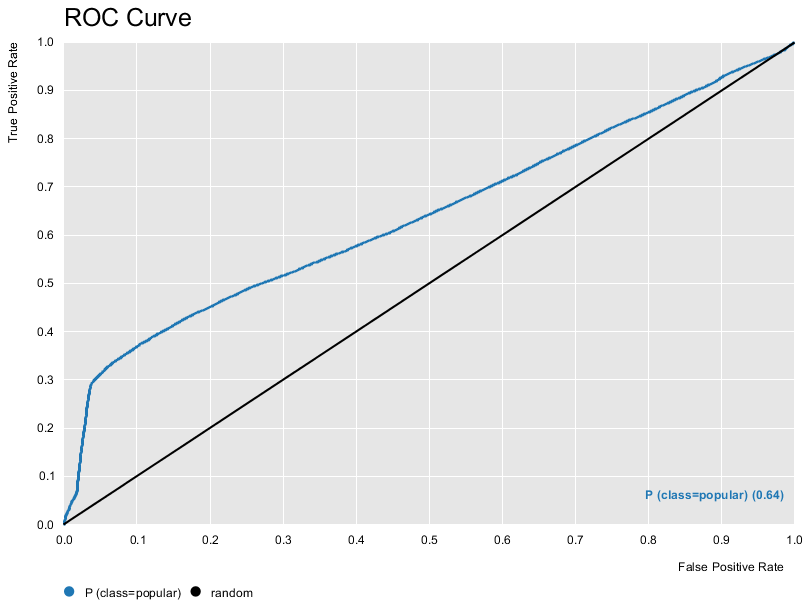
\includegraphics[scale=0.38]{rc-svm.png}  %el parámetro scale permite agrandar o achicar la imagen. En el nombre de archivo puede especificar dirctorios
	\caption{Curva ROC SVM} 
	\label{fig:rocsvm}
\end{figure}

\subsection{Gradient Boosting}

Gradient Boosting era el algoritmo que tenía el mejor comportamiento en este problema según el análisis anterior. Al alterar los datos, podría darse el caso de que ya no fuera tan bueno. Sin embargo, los datos reflejan que sigue siendo el más útil:

\begin{table}[H]
	\centering
	\begin{tabular}{|l|l|l|l|l|l|l|}
		\hline
		Row ID          & TPR   & TNR   & AUC   & Valor-F1 & G-mean   & Accuracy \\ \hline
		no\_popular\_np & 0.977 & 0.092 &       & 0.872    & 0.299806 &          \\ \hline
		no\_popular\_p  & 0.873 & 0.71  &       & 0.808    & 0.787292 &          \\ \hline
		popular\_np     & 0.092 & 0.977 & 0.716 & 0.157    & 0.299806 &          \\ \hline
		popular\_p      & 0.71  & 0.873 & 0.868 & 0.773    & 0.787292 &          \\ \hline
		Overall\_np     &       &       &       &          &          & 0.778    \\ \hline
		Overall\_p      &       &       &       &          &          & 0.792    \\ \hline
	\end{tabular}
\end{table}

Encontramos en ellos un gran crecimiento tanto en AUC como en accuracy. Veamos las curvas ROC.

\begin{figure}[H]
	\begin{subfigure}{.5\textwidth}
		\centering
		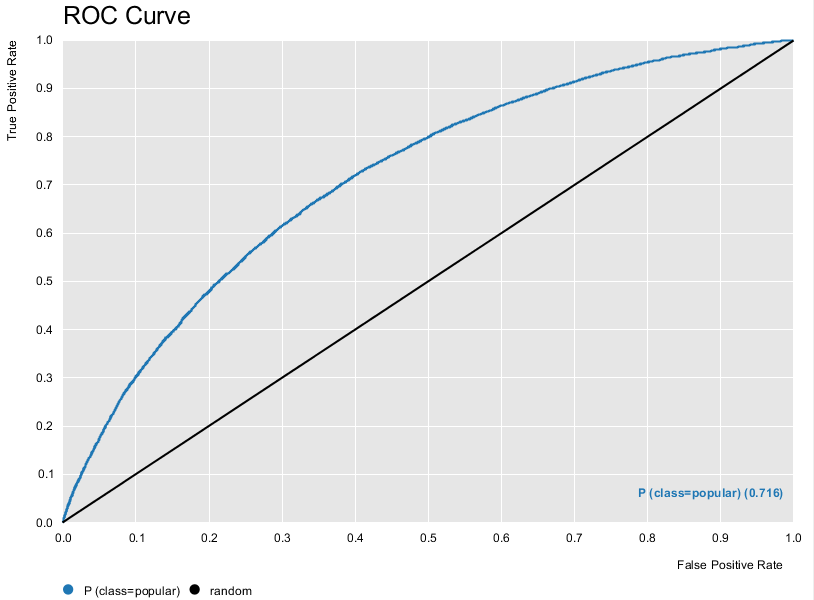
\includegraphics[width=.4\linewidth]{roc-gb-p.png}
		\caption{Curva ROC del Gradient Boosting (previo)}
		\label{fig:rcgbp}
	\end{subfigure}%
	\begin{subfigure}{.5\textwidth}
		\centering
		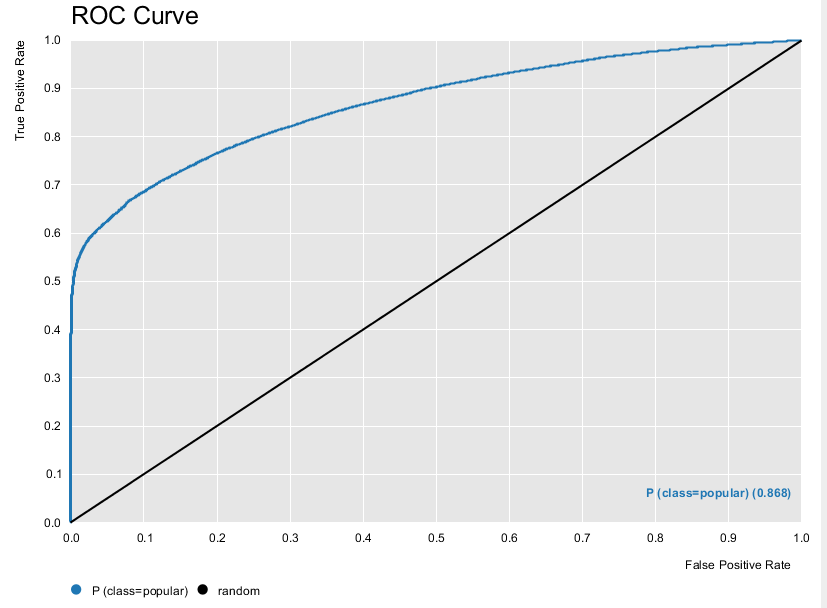
\includegraphics[width=.4\linewidth]{roc-gb.png}
		\caption{Curva ROC del Gradient Boosting (posterior)}
		\label{fig:rcgb}
	\end{subfigure}
	\caption{Curvas ROC del Gradient Boosting}
	\label{fig:gb}
\end{figure}

\subsection{MLP}

Tratamos finalmente el último algoritmo. Si estudiamos los datos previos al preprocesado, como consecuencia del gran desbalanceo que tenía el dataset, para la clase positiva TPR=0 Y TNR=1 (al contrario para la clase negativa). Esto hacía que la clasificación fuera mala. Tras el preprocesado, se equilibran las tasas TPR y TNR pero sigue teniendo malos resultados.

\begin{table}[H]
	\centering
	\begin{tabular}{|l|l|l|l|l|l|l|}
		\hline
		Row ID          & TPR   & TNR   & AUC   & Valor-F1 & G-mean   & Accuracy \\ \hline
		no\_popular\_np & 1     & 0     &       & 0.874    & 0        &          \\ \hline
		no\_popular\_p  & 0.228 & 0.786 &       & 0.316    & 0.423329 &          \\ \hline
		popular\_np     & 0     & 1     & 0.496 & 0        & 0        &          \\ \hline
		popular\_p      & 0.786 & 0.228 & 0.51  & 0.615    & 0.423329 &          \\ \hline
		Overall\_np     &       &       &       &          &          & 0.776    \\ \hline
		Overall\_p      &       &       &       &          &          & 0.507    \\ \hline
	\end{tabular}
\end{table}

El área bajo la curva apenas cambia, como podemos aprecias en la comparativa de curvas ROC:

\begin{figure}[H]
	\begin{subfigure}{.5\textwidth}
		\centering
		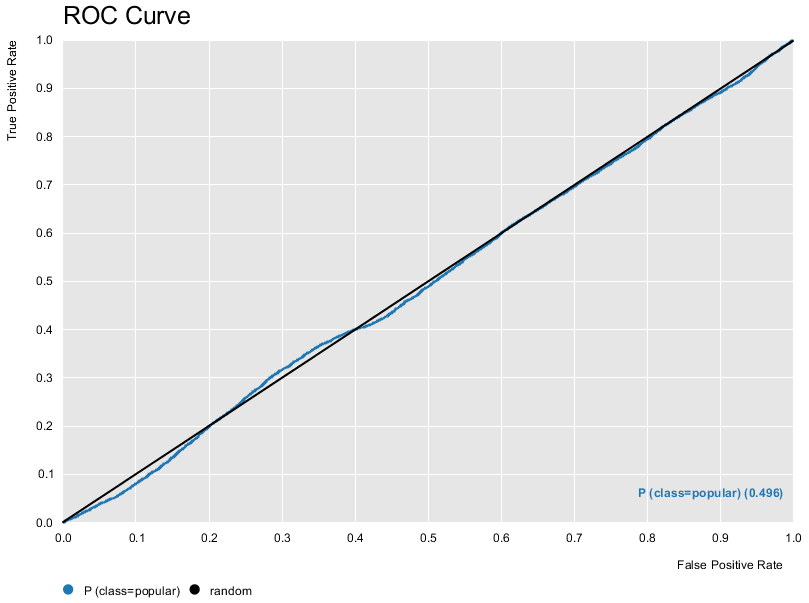
\includegraphics[width=.4\linewidth]{roc-rn-p.png}
		\caption{Curva ROC del MLP (previo)}
		\label{fig:rcmlpp}
	\end{subfigure}%
	\begin{subfigure}{.5\textwidth}
		\centering
		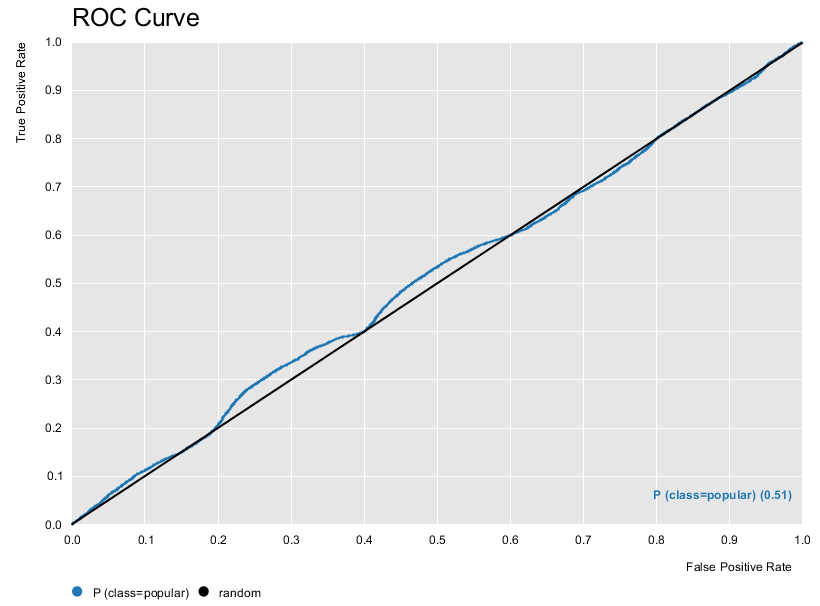
\includegraphics[width=.4\linewidth]{roc-mlp.png}
		\caption{Curva ROC del MLP (posterior)}
		\label{fig:rcmlp}
	\end{subfigure}
	\caption{Curvas ROC del MLP}
	\label{fig:mlp}
\end{figure}

\subsection{Comparativa general}

En la siguiente tabla resumo todo lo expuesto antes:

\begin{table}[H]
	\centering
	\begin{tabular}{|l|l|l|l|l|}
		\hline
		Row ID            & Accuracy\_np & AUC\_np & Accuracy\_p & AUC\_p   \\ \hline
		C4.5 KNIME        & 0.7         & 0.556  & 0.753    & 0.811 \\ \hline
		Random Forest     & 0.778       & 0.699  & 0.768    & 0.854 \\ \hline
		KNN               & 0.731       & 0.547  & 0.711    & 0.789 \\ \hline
		Naïve-Bayes       & 0.563       & 0.643  & 0.619    & 0.674 \\ \hline
		SVM               &             &        & 0.634    & 0.64  \\ \hline
		Gradient Boosting & 0.778       & 0.716  & 0.792    & 0.868 \\ \hline
		MLP               & 0.776       & 0.496  & 0.507    & 0.51  \\ \hline
	\end{tabular}
\end{table}

\begin{figure}[H] %con el [H] le obligamos a situar aquí la figura
	\centering
	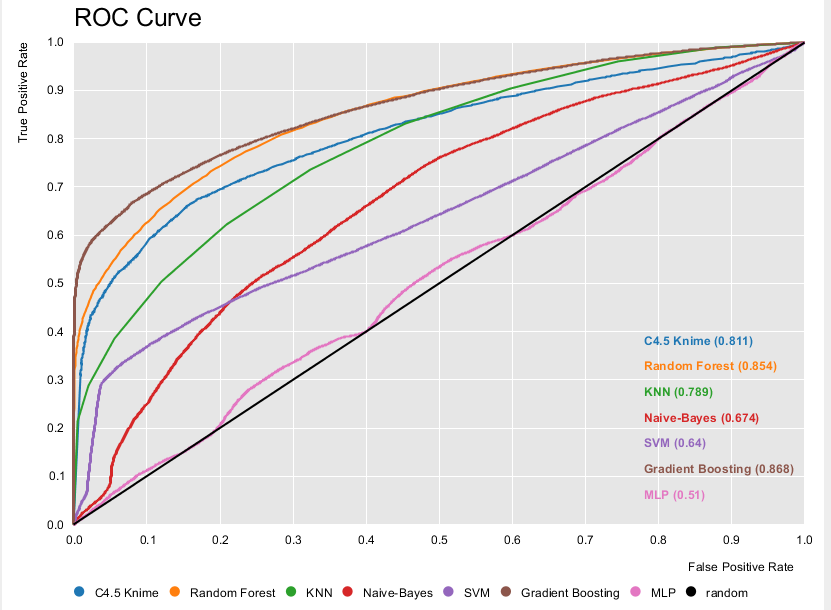
\includegraphics[scale=0.4453]{roc-global.png}  %el parámetro scale permite agrandar o achicar la imagen. En el nombre de archivo puede especificar directorios
	\caption{Comparativa de Curvas ROC} 
	\label{fig:rocglobal}
\end{figure}

Por tanto, se puede ver que Gradient Boosting es el mejor algoritmo en cuanto a comportamiento, dado que Boosting está indicado para problemas con un gran sesgo y una varianza baja (\cite{gb}, \cite{gb1}). Precisamente en el preprocesamiento he minimizado la varianza para seleccionar características. De cerca le siguen Random Forest y C4.5. Este último es meritorio, ya que tras el preprocesamiento se ha reducido muchísimo el número de reglas que genera, aumentando la interpretabilidad. Como vemos, los algoritmos basados en reglas tienen un decente comportamiento con este dataset. El resultado de MLP indica que necesita un procesado de los datos más específico. No obstante, en términos pedagógicos ha sido interesante aprender a configurar una red neuronal, a pesar del bajo rendimiento adquirido. 


Por otra parte, de las 52 características que conformaban el dataset, el preprocesado informa de que sólo 12 son más o menos relevantes. Son las siguientes: \textit{data-channel-is-entertainment, data-channel-is-bus, data-channel-is-socmed, data-channel-is-tech, data-channel-is-world, kw-min-avg, LDA-01, LDA-03, max-positive-popularity, title-subjetivity, abs-title-subjetivity, abs-title-sentiment-polarity}, es decir, son relevantes las características referentes al canal de comunicación, a los valores del algoritmo Latent Dirichlet Allocation (\cite{lda}) y la polaridad/subjetividad de los títulos y resúmenes. 

%----------------------------------------------------------------------------------------
%	Contenido adicional
%----------------------------------------------------------------------------------------

\newpage

\section{Contenido adicional}

\subsection{Sobre sobreajuste y Random Forest}
Tras toda la discusión anterior, y para cerrar el documento, quiero tratar el sobreajuste del clasificador Random Forest. Este tema ha sido ampliamente estudiado en la literatura (por ejemplo, \cite{Breiman2001}). Para hacer mi pequeño experimento, defino un workflow con validación cruzada de 2 particiones (me dan errores con un número mayor de ellas) de forma que los conjuntos de training y test son iguales:

 \begin{figure}[H] %con el [H] le obligamos a situar aquí la figura
 	\centering
 	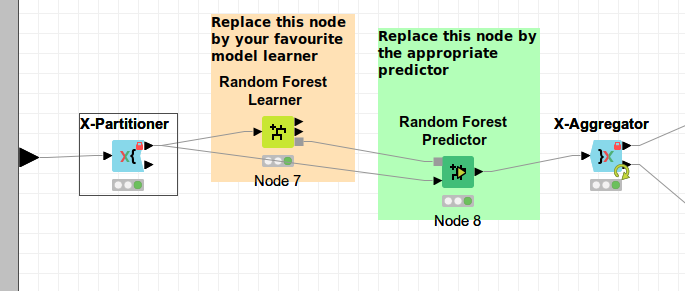
\includegraphics[scale=0.4453]{exp1.png}  %el parámetro scale permite agrandar o achicar la imagen. En el nombre de archivo puede especificar directorios
 	\caption{Configuración de la validación cruzada} 
 	\label{fig:exp}
 \end{figure}

Los resultados no decepcionan: Accuracy=1 y AUC=1. \\

Sin embargo, cuando diferenciamos los conjuntos de training y test, Accuracy=0.77 y AUC=0.697. Por tanto, se da un sobreajuste. Podemos paliar los efectos de dicho overfitting retocando los parámetros y llegando a unos niveles de AUC de entorno a 0.75.

\newpage
\section{Bibliografía}

%------------------------------------------------

\bibliography{citas} %archivo citas.bib que contiene las entradas 
\bibliographystyle{plain} % hay varias formas de citar

\end{document}
